
\section{O HARDWARE DO ROB{\^O}}

Ap{\'o}s o contato com outras equipes e pesquisa em rela{\c c}{\~a}o aos materiais, decidiu-se por reformular a estrutura 
dos rob{\^o}s. Visando a simplifica{\c c}{\~a}o das montagens, bem como agilidade na manuten{\c c}{\~a}o, os rob{\^o}s 
adquiriram um escopo modular. Dessa forma, cada conjunto de componentes respons{\'a}vel por um setor do rob{\^o} {\'e} 
acoplado a um dos m{\'o}dulos separadamente. Assim, caso algum dos m{\'o}dulos apresente problemas de execu{\c c}{\~a}o, 
ele pode ser trocado por outro igual reserva, sem que haja excessiva perda de tempo. Inicialmente, cogitou-se a 
exist{\^e}ncia de tr{\^e}s m{\'o}dulos: os motores junto das rodas; a bateria; e a placa controladora com os componentes
discretos. O m{\'o}dulo da placa controladora, que cont{\'e}m, entre outros componentes, o Arduino Nano[6], {\'e} agora 
livre de fios e componentes soldados diretamente ao fenolite. Novamente em busca de agilidade na manuten{\c c}{\~a}o, 
somente soquetes e caixas de pinos foram soldadas diretamente na placa, de modo que os componentes s{\~a}o remov{\'i}veis
e de f{\'a}cil substitui{\c c}{\~a}o. A bateria, que {\'e} empregada agora no lugar das pilhas AA de vers{\~o}es 
anteriores, ocupa sozinha, junto de um pequeno circuito de verifica{\c c}{\~a}o de carga, o segundo m{\'o}dulo. Isso 
ocorre devido ao trabalho necess{\'a}rio para carreg{\'a}-la. Diferentemente das pilhas, onde bastava uma fonte de 
alimenta{\c c}{\~a}o para recarregar o rob{\^o}, a bateria de l{\'i}tio exige um circuito pr{\'o}prio externo ao rob{\^o} 
para carregar adequadamente. O circuito verificador de carga {\'e} respons{\'a}vel por impedir que a bateria chegue a 
n{\'i}veis muito baixos, o que prejudicaria seu desempenho. O {\'u}ltimo dos m{\'o}dulos {\'e} composto pelos motores e 
rodas. A {\'u}nica diferen{\c c}a desse sistema para o anterior {\'e} o di{\^a}metro das rodas, que cresceu 2mm, e seu 
acabamento.

O rob{\^o} foi constru{\'i}do tem um Arduino Nano[6] como m{\'o}dulo de controle. Este m{\'o}dulo recebe, via um 
transceptor de r{\'a}dio NRF24L01, os comandos de velocidade desejados para cada uma das rodas. O Arduino aciona os 
motores utilizando modula{\c c}{\~a}o por largura de pulso PWM (Pulse-Width Modulation) atrav{\'e}s 
de uma placa equipada com o componente por um circuito impresso L293.

A rota{\c c}{\~a}o das rodas, e consequentemente o deslocamento
do rob{\^o}, s{\~a}o determinados por sensores TCRT5000, que
codificam o movimento de dentes reflexivos fixados às rodas
em pulsos enviados ao Arduino. Esses pulsos s{\~a}o contados e
servem de realimenta{\c c}{\~a}o ao acionamento direcionado a cada
motor. Um esquema representativo da eletr{\^o}nica do rob{\^o} pode
ser apreciado na Fig 10 .

Do lado do computador pessoal, o envio dos comandos
tamb{\'e}m ocorre atrav{\'e}s de um circuito controlado por um
Arduino Nano[6] conectado a uma interface USB. Este Arduino
recebe os comandos a ser enviados aos rob{\^o}s e os transmite por
meio de um transceptor de r{\'a}dio NRF24L01 id{\^e}ntico ao
utilizados nos rob{\^o}s.

% FIGURA 10
\begin{figure}[!htb]
\centering
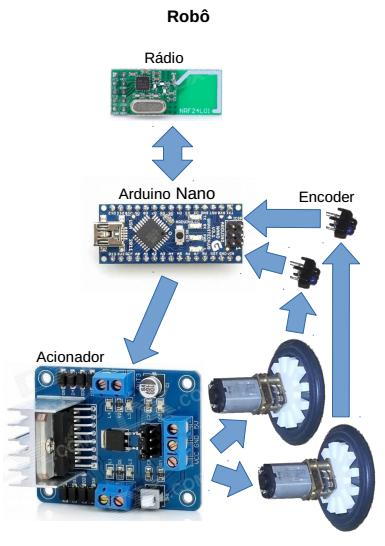
\includegraphics[scale=0.7]{robo.png}
\caption{Esquema dos componentes eletr{\^o}nicos usados em cada rob{\^o}.}
\label{Rotulo}
\end{figure} 
